\section{Experiment Outline}\label{section:experiment_outline}

In the following subsections, we will briefly explain the underlying reasons for the way we have setup our experiments.

\subsection{Method Selection}

These experiments are meant to address proposals \textbf{1)} (performance comparison of multiple tag-predictions approaches in two very different datasets) and \textbf{2)} (comparing the MIMLSVM tag prediction method using sparse and dense features). In order to have representative and non-biased experiments, we have chosen to use methods that were \textbf{a)} widely used in practice, \textbf{b)} different from other methods or \textbf{c)} both.

\subsection{Hyperparameter Tuning}

As is commonplace in most machine learning tasks, we have, for each experiment, tried a combination of hyperparameters for each method we have applied. We have used \textit{grid search}, probably the most common way to conduct hyperparameter search, to search for good configurations for the problems at hand. The actual search was done on a sample (generally 30\% of the full data) and the victor parameters used to train the model on the full datasets.

With respect to text-specific machine-learning, there is also the question of how to tune some feature extraction procedures. Once again, we have tried to emulate what has been done by other authors we have reviewed while also taking into account standard practice in the Natural Language Processing (NLP) field. We consider the two most important choices to be \textbf{a)} the number of words to use in BOW representation and \textbf{b)} the number of dimensions to use for word embeddings. We have conducted two simple comparisons to help us make appropriate choices for these parameters, taking into account both accuracy but also more practical matters such as training time and memory needed.

\begin{figure}[H]
    \begin{subfigure}{0.5\textwidth}
        \centering
    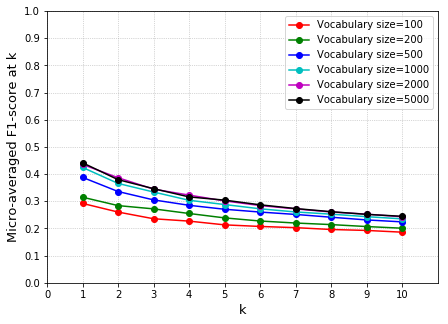
\includegraphics[width=0.8\textwidth]{chapters/05_experiments/images/comparison-vocabulary-size.png}
    \caption{Comparing performance using different vocabulary sizes (OvR SVM).}
    \label{fig:vocabulary_size_comparison}
    \end{subfigure}
    \begin{subfigure}{0.5\textwidth}
        \centering
    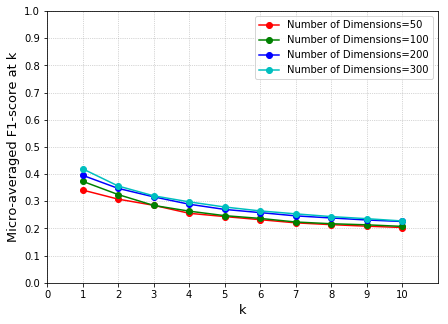
\includegraphics[width=0.8\textwidth]{chapters/05_experiments/images/comparison-number-of-dimensions.png}
    \caption{Comparing performance using different embedding dimensions. (OvR SVM)}
    \label{fig:embedding_dimension_comparison}
    \end{subfigure}
    \caption{Comparing choice of hyperparameters for feature extraction. Using Dataset 2 for illustrative purposes.}
\end{figure}

Based on the above tests, we have concluded that using a vocabulary with only 500 as the number of words and 100 as the embedding dimension represents a good trade-off between performance and training time and complexity. In other words, we consider these to be enough to enable comparing methods while not incurring long training times and extreme memory consumption.

\subsection{Metrics and Evaluation}

For measuring the output of the selected methods, we have chosen to use \textbf{micro-averaged F1-score @k}.\footnote{More detailed information on this and other metrics and be found in \cite{sokolova_and_napalme_2009}.}

This measure was chosen due to the problem we wish to consider (namely, label ranking) and the way we want to average the results over a given dataset. In addition, this metric is commonly used in articles we have reviewed.

The F1-score (a particular case of the more general \textit{F-measure}, where $\beta$ equals 1) is widely used in information retrieval problems related to search or ranking of results; it is the harmonic mean of precision and recall, given by:

\begin{equation}
F_1 = 2 \cdot \frac{precision \cdot recall}{precision + recall} 
\end{equation}

which can be also written in terms of generic error metrics:

\begin{equation}
F_1 = \frac{2 \cdot true \ positive}{2 \cdot true \ positive + false \ negative + false \ positive} 
\end{equation}\\

With regards to \textit{micro-averaging}, it refers to the way we report results for the whole dataset, be it training or validation.

When \textit{macro-averaging} is used, equal weight is given to every class (label) in the dataset, which means that classes which occur only very rarely are given the same weight and very common classes when the full metrics over the dataset are calculated.

On the other hand, with \textit{micro-averaging}, the individual metrics (true positive, true negative, false positive and false negative) are aggregated over the whole dataset, which is preferable in cases (such as ours) where the dataset is highly unbalanced. \footnote{I.e. some labels appear much more often than others.}  

Finally, when metrics $@k$ are considered, it simply means that only the results up to the $k$-th position are taken into account when gathering the results:

\begin{equation}
F_1\ @k = \frac{2 \cdot true \ positive\ @k}{2 \cdot true \ positive\ @k + false \ negative\ @k + false \ positive\ @k} 
\end{equation}\\

This gives a more complete view of how the classifier works at different precision/recall levels, and can be easily visualized via graphical charts.